
\section{Là où tout commence : Hello World}
Pour commencer, nous allons créer un programme simple qui affiche "Hello World" à l'écran.

\begin{UPSTIManipulation}{Hello World}
    \begin{minipage}{.7\textwidth}
        \begin{itemize}
            \item Ouvrez un éditeur Scratch sur le \href{https://scratch.mit.edu/projects/editor}{site du MIT}
            \item Dans la palette de blocs, trouvez le bloc "Quand le drapeau vert est cliqué".
            \item Ajoutez le bloc "dire Bonjour pendant 2 secondes" sous le bloc précédent.
            \item Modifier le texte pour Hello World
            \item Cliquez sur le drapeau vert pour exécuter votre programme.   
            \item Vous devriez obtenir le résultat ci-contre. 
        \end{itemize}
    \end{minipage}\hfill
    \begin{minipage}{.25\textwidth}
        \begin{center}
            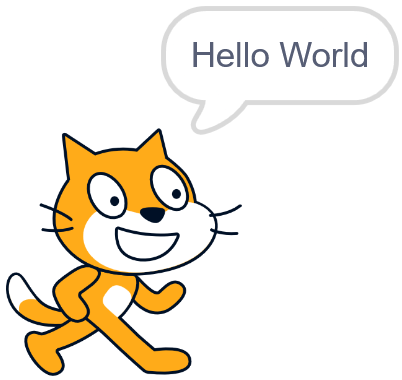
\includegraphics[width=\linewidth]{scratch_says_hello.png}
        \end{center}
    \end{minipage}
\end{UPSTIManipulation}


\begin{UPSTIinfor}{Besoin d'aide ?}
    Scratch est bien documenté sur son site internet : \href{https://scratch.mit.edu/help}{documentation de Scratch} Vous pouvez également trouver des tutoriels en ligne. \\
Le bloc \raisebox{-0.3\height}{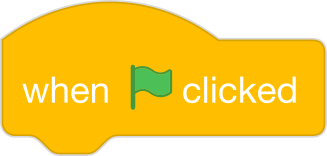
\includegraphics[height=3em]{when-flag-clicked.png}} se trouve dans la catégorie "Événements" ("Events").\\
Le bloc \raisebox{-0.3\height}{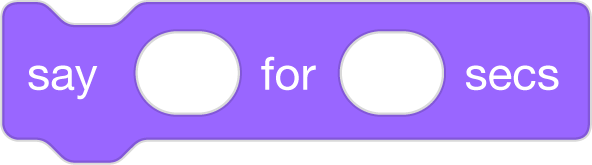
\includegraphics[height=3em]{say-secs.png}} se trouve dans la catégorie "Apparence".\\
\end{UPSTIinfor}

